% много редких events
%Log-likelihood tests
%The practical effect of this improvement is that
%statistical textual analysis can be done effectively with very much smaller volumes of
%text than is necessary for conventional tests based on assumed normal distributions,
%and it allows comparisons to be made between the significance of the occurrences of
%both rare and common phenomenon.
%
%
%The likelihood ratio for a hypothesis is the ratio of the maximum value of the likelihood
%function over the subspace represented by the hypothesis to the maximum value of
%the likelihood function over the entire parameter space.
%
%
%The particularly important feature of likelihood ratios is that the quantity -2 log )~
%is asymptotically X 2 distributed with degrees of freedom equal to the difference in
%dimension between f~ and f~0. Importantly, this asymptote is approached very quickly
%in the case of binomial and multinomial distributions.
%
%If the null hypothesis holds, then the log-likelihood ratio is asymptotically X 2 distributed with k/2 - 1 degrees of freedom. When j is 2 (the binomial), -2 log )~ will be
%X 2 distributed with one degree of freedom.
%
%The likelihood ratio -> the logarithm of the likelihood ratio ->
%
%https://ucrel.lancs.ac.uk/llwizard.html


\documentclass[svgnames]{beamer}
%\mode<presentation>
%{
%  \usetheme[titleformat=smallcaps,numbering=fraction,progressbar=frametitle]{metropolis}
%  \usecolortheme[light,accent=orange]{solarized}
%  %\usecolortheme[named=Goldenrod]{structure}
%  % or ...
%
%  \setbeamercovered{transparent}
%  % or whatever (possibly just delete it)
%}


% \usepackage{mathtext}
\usepackage[utf8]{inputenc}
\usepackage[english,russian]{babel}
\usepackage{cmap}
\hypersetup{unicode=true}
\graphicspath{{images/}{slides/images}}


\title[CMTA 03] % (optional, use only with long paper titles)
{Contrastive analysis}

\subtitle
{Computational Methods for Text Analysis} % (optional)

\author%[Author, Another] % (optional, use only with lots of authors)
{Pestova Alena Sergeevna}
% - Use the \inst{?} command only if the authors have different
%   affiliation.

\institute%[Universities of Somewhere and Elsewhere] % (optional, but mostly needed)
{НИУ ВШЭ Санкт-Петербург}
% - Use the \inst command only if there are several affiliations.
% - Keep it simple, no one is interested in your street address.

\date%[Short Occasion] % (optional)
{25.09.2021 / 03}

\subject{natural language processing, text mining}
% This is only inserted into the PDF information catalog. Can be left
% out. 


%\AtBeginSubsection[]
%{
%  \begin{frame}<beamer>[plain]{План}
%    \tableofcontents[sectionstyle=show/hide,subsectionstyle=show/shaded/hide]
%  \end{frame}
%}

\newcommand{\tb}[1]{\colorbox{yellow}{#1}\space}
\newcommand{\Sp}[1]{\colorbox{green}{#1}\space}
\newcommand{\Sn}[1]{\colorbox{red}{#1}\space}


\begin{document}

\begin{frame}
  \titlepage
\end{frame}


\begin{frame}
  \frametitle{Corpus-based contrastive analysis}
  The task is to extract vocabulary specific to a given corpus
  \begin{itemize}
  \item \textbf{Reference corpus} represents word usage in a language in general or in some subject area
  \item Build the frequency lists for the corpus of interest and the reference corpus
  \item Sort words by the difference in frequency of the studied corpus with the reference corpus
  \item Keywords of the studied corpus are at the top of the list - the words that are more specific to this particular corpus
  \end{itemize}
\end{frame}


\begin{frame}
  \frametitle{Keywords of the corpus}
  \begin{block}{Simple maths (by Adam Kilgarriff)}
  «this word is twice as common in this corpus as in that corpus»
\end{block}
\begin{itemize}
\item The simplest way
  \begin{itemize}
  \item Normalize the frequencies
    \begin{itemize}
    \item metric Instances per million (IPM)
    \end{itemize}
  \item Calculate the ratio of the normalized frequencies
  \item Sort the lists by the calculated reatio
  \end{itemize}
\end{itemize}
\end{frame}

\begin{frame}
  
For example:
\begin{itemize}
\item Two corpora, the size of each corpus is one million tokens
\item We do not need to normalize frequencies
\item[Fc] focus corpus — the studies corpus
\item[Rc] reference corpus
\end{itemize}
\end{frame}

\begin{frame}
  \frametitle{Problem 1:  we cannot divide by 0}
  \begin{tabular}[l]{lccc}
    word & fc & rc & ratio \\
    \hline
    rarity & 10 & 0 &  ? \\
    stir & 100 & 0 &  ? \\
    yummy & 1000 & 0 &  ? \\
  \end{tabular}
\end{frame}

\begin{frame}

Standard solution - add 1:
  \begin{tabular}[l]{lccc}
    word & fc & rc & ratio \\
    \hline
    rarity & 11 & 1 &  11 \\
    stir & 101 & 1 &  101 \\
    yummy & 1001 & 1 &  1001 \\
  \end{tabular}
\end{frame}

\begin{frame}
  \frametitle{Problem 2: there are two many big ratios because of rare words}
  The frequency is also important.   Solution: add n.

  \begin{itemize}
  \item $n=1$

  \begin{tabular}[l]{lcccccc}
    word & fc & rc & fc+n & rc+n & ratio & rank \\
    \hline
    rare & 10 & 0 & 11 & 1 & 11,00 & 1 \\
    sometimes & 200 & 100 & 201 & 101 & 1,99 & 2 \\
    frequent & 12000 & 10000 & 12001 & 10001 & 1,20 & 3 \\
  \end{tabular}
  
  \item $n=100$

  \begin{tabular}[l]{lcccccc}
    word & fc & rc & fc+n & rc+n & ratio & rank \\
    \hline
    rare & 200 & 300 & 300 & 400 & 0.75 & 1 \\
    sometimes & 10 & 0 & 110 & 100 & 1,10 &  2 \\
    frequent & 12000 & 10000 & 12100 & 10100 & 1,20 & 1 \\
  \end{tabular}

  \end{itemize}
  
\end{frame}


\begin{frame}
  \frametitle{Normality and words distribution}

In the paradigm of the standard statistical tests, there were problems with comparing frequiencies

  \begin{itemize}
  \item The normality assumption is unlikely in the case of words frequency distribution
  \item There are too many rare events in the language (remember Zipf's Law)
  \item Inapplicability of tests based on the assumption of normality (e.g. chi-square), at least to rare events (frequency < 5)
  \end{itemize}
\end{frame}


\begin{frame}
  \frametitle{Dunning log-likelihood: motivation}
  \framesubtitle{Log likelihood ratio}

A way to incorporate word frequencies into the statistical test paradigm:

  \href{https://aclanthology.org/J93-1003.pdf}{Ted Dunning "Precise
    Surprise and Coincidence Statistics Methods (1994)}
  \begin{itemize}
  \item Dunning log-likelihood is less dependent on an assumption of the distribution normality
  \item Therefore, it does not overestimate the detection of rare events so much and
    can be used for evaluation of not only the most frequent words
  \end{itemize}
\end{frame}


\begin{frame}
  \frametitle{Dunning log-likelihood: formulas}
  \begin{tabular}[c]{|p{.3\textwidth}|c|c|c|}
    \hline
   & Corpus 1 & Corpus 2 & Total \\
    \hline
    Word Frequency & a & b & a+b \\
    \hline
    Frequency of other words & c-a & d-b & c+d-a-b \\
    \hline
    Total & c & d & c+d \\
    \hline
  \end{tabular}

\bigskip
  Expected frequencies:
  \begin{itemize}
  \item[E1] $\frac{c}{c+d}(a+b)$
  \item[E2] $\frac{d}{c+d}(a+b)$
  \end{itemize}

  \begin{equation}
    LL = G^2 = 2 (a \log (a/E1) + b \log (b/E2) ) 
  \end{equation}
\end{frame}

\begin{frame}
  If we calculate the log-likelihood ratio test for two words in two corpora, then


    $$G^2 \approx X^2(1)$$


      We can calculate statistical significance of the difference (on the level of significance 0.05):

      $$\text{p-value}: P(X^2 >= 3.84)$$

      $$\text{CDF}(3.84) = 0.95 \text{for} X^2$$

\end{frame}

\begin{frame}
  \frametitle{Log-Likelihood ratio}

  \begin{itemize}
    \item The practical effect of this improvement is that  statistical textual analysis can be done
  effectively with very much smaller volumes of text than is necessary for conventional tests based on assumed normal distributions
  \item It allows comparisons to be made between the significance of the occurrences of both rare and common phenomenon.
  \item More sensitive to frequent events (words) than to less frequent one [underestimates the degree of difference for less frequent words]
  \end{itemize}
\end{frame}

\begin{frame}{Log-odds}

  $$\text{LR} = \log\frac{(a/sum(a))}{(b/sum(b))}$$

\end{frame}


\begin{frame}
  \begin{itemize}
    \item $G^2$ for stat. significance and log-odds for effect size, sorting by log-odds
    \item sorting by log-odds and/or $G^2$, finding a threshold for cutting lists
\end{itemize}
\end{frame}


%\begin{frame}
%  \frametitle{Сonditional Probability}
%$$
%    P(Event|Condition)
%$$
%\end{frame}
%
%\begin{frame}
%  \frametitle{Сonditional Probability}
%  \begin{equation}
%    P(B|A) = \frac{P(B \land A)}{P(A)}
%  \end{equation}
%
%  $$
%    P(\text{intelligence}|\text{artificial}) =
%    \frac{P(\text{artificial intelligence})}{P(\text{artificial})}
%    =$$
%
%    $$
%    = \frac{\frac{4}{46804371}}{\frac{121}{46804371}} = \frac{4}{121} = 0.033$$
%\end{frame}

%\begin{frame}
%  \frametitle{Pointwise mutual information}
%  \begin{columns}
%    \column{.5\textwidth}
%    PMI
%
%  $$
%  pmi(x;y) = log \frac{p(x,y)}{p(x)p(y)} =
%  $$
%  $$
%  = log \frac{p(x|y)}{p(x)} =
%  $$
%  $$
%  = log \frac{p(y|x)}{p(y)}
%  $$
%
%  Positive PMI
%
%    $$
%    ppmi(x;y) = max(pmi(x;y),0)
%    $$
%    \column{.5\textwidth}
%  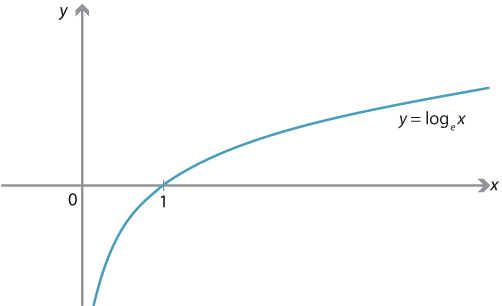
\includegraphics[width=\textwidth]{log}
%  \end{columns}
%\end{frame}

%\begin{frame}
%  \frametitle{The problem of PMI}
%  \begin{itemize}
%  \item Very sensitive to rare events that are highly informative relative to each other (words always occur together)
%    [increase the degree of difference for rare words]
%  \end{itemize}
%\end{frame}


%\begin{frame}
%  \frametitle{The probability of independent events}
%  Independent events - the occurrence of one does not change the probabilities
%  another.
%  \begin{equation}
%    P(B|A) = P(B) \quad | P(B) > 0
%  \end{equation}
%
%  \begin{equation}
%    P(B \cap A) = P(A) \cdot P(B)
%  \end{equation}
%\end{frame}

%\begin{frame}
%  \frametitle{Joint Probability}
%  \structure{For the independent events A и B}:
%
%    $p(\text{A and B}) = p(A)p(B)$ \quad{} | $p(B|A) = p(B)$
%
%    \bigskip
%
%  \pause
%  \structure{In general case}:
%
%   $p(\text{A and B}) = p(A)p(B|A)$ \quad{} | $p(B|A) \neq p(B)$
%\end{frame}

%\begin{frame}
%  \frametitle{Bayes rule}
%  \begin{equation}
%    P(A|B) = \frac{P(B|A)P(A)}{P(B)}
%  \end{equation}
%  \pause
%  \begin{equation}
%    posterior = \frac{likelihood \cdot prior}{evidence}
%  \end{equation}
%\end{frame}


\begin{frame}
  \frametitle{tidylo by Julia Silge: weighted log odds}
  \begin{enumerate}
  \item Log odds ratio:
    $$
    O_1 = \frac{f_{(w,c1)}}{N_{c1}-f_{(w,c1)}}
    $$
    $$
    O_2 = \frac{f_{(w,c2)}}{N_{c2}-f_{(w,c2)}}
    $$
    $$
    LO = log \frac{O_1}{O_2}
    $$
  \item Weighted by uninformative Dirichlet prior:
    $$
    \delta =
    \frac{\frac{f_{(w,c1)}+\alpha_{(w,c1)}}{N_{c1}+\alpha_{c1}-f_{(w,c1)}-\alpha_{(w,c1)}}}{\frac{f_{(w,c2)}+\alpha_{(w,c2)}}{N_{c2}+\alpha_{c2}-f_{(w,c2)}-\alpha{(w,c2)}}}
    $$
  \end{enumerate}

  package tidylo in R
\end{frame}


\end{document}
